% Options for packages loaded elsewhere
\PassOptionsToPackage{unicode}{hyperref}
\PassOptionsToPackage{hyphens}{url}
%
\documentclass[
]{article}
\usepackage{amsmath,amssymb}
\usepackage{iftex}
\ifPDFTeX
  \usepackage[T1]{fontenc}
  \usepackage[utf8]{inputenc}
  \usepackage{textcomp} % provide euro and other symbols
\else % if luatex or xetex
  \usepackage{unicode-math} % this also loads fontspec
  \defaultfontfeatures{Scale=MatchLowercase}
  \defaultfontfeatures[\rmfamily]{Ligatures=TeX,Scale=1}
\fi
\usepackage{lmodern}
\ifPDFTeX\else
  % xetex/luatex font selection
\fi
% Use upquote if available, for straight quotes in verbatim environments
\IfFileExists{upquote.sty}{\usepackage{upquote}}{}
\IfFileExists{microtype.sty}{% use microtype if available
  \usepackage[]{microtype}
  \UseMicrotypeSet[protrusion]{basicmath} % disable protrusion for tt fonts
}{}
\makeatletter
\@ifundefined{KOMAClassName}{% if non-KOMA class
  \IfFileExists{parskip.sty}{%
    \usepackage{parskip}
  }{% else
    \setlength{\parindent}{0pt}
    \setlength{\parskip}{6pt plus 2pt minus 1pt}}
}{% if KOMA class
  \KOMAoptions{parskip=half}}
\makeatother
\usepackage{xcolor}
\usepackage[margin=1in]{geometry}
\usepackage{longtable,booktabs,array}
\usepackage{calc} % for calculating minipage widths
% Correct order of tables after \paragraph or \subparagraph
\usepackage{etoolbox}
\makeatletter
\patchcmd\longtable{\par}{\if@noskipsec\mbox{}\fi\par}{}{}
\makeatother
% Allow footnotes in longtable head/foot
\IfFileExists{footnotehyper.sty}{\usepackage{footnotehyper}}{\usepackage{footnote}}
\makesavenoteenv{longtable}
\usepackage{graphicx}
\makeatletter
\def\maxwidth{\ifdim\Gin@nat@width>\linewidth\linewidth\else\Gin@nat@width\fi}
\def\maxheight{\ifdim\Gin@nat@height>\textheight\textheight\else\Gin@nat@height\fi}
\makeatother
% Scale images if necessary, so that they will not overflow the page
% margins by default, and it is still possible to overwrite the defaults
% using explicit options in \includegraphics[width, height, ...]{}
\setkeys{Gin}{width=\maxwidth,height=\maxheight,keepaspectratio}
% Set default figure placement to htbp
\makeatletter
\def\fps@figure{htbp}
\makeatother
\setlength{\emergencystretch}{3em} % prevent overfull lines
\providecommand{\tightlist}{%
  \setlength{\itemsep}{0pt}\setlength{\parskip}{0pt}}
\setcounter{secnumdepth}{5}
\usepackage{booktabs}
\usepackage{fontspec}
\usepackage{multirow}
\usepackage{multicol}
\usepackage{colortbl}
\usepackage{hhline}
\newlength\Oldarrayrulewidth
\newlength\Oldtabcolsep
\usepackage{longtable}
\usepackage{array}
\usepackage{hyperref}
\usepackage{float}
\usepackage{wrapfig}
\ifLuaTeX
  \usepackage{selnolig}  % disable illegal ligatures
\fi
\IfFileExists{bookmark.sty}{\usepackage{bookmark}}{\usepackage{hyperref}}
\IfFileExists{xurl.sty}{\usepackage{xurl}}{} % add URL line breaks if available
\urlstyle{same}
\hypersetup{
  pdftitle={The Sense of Belonging Scale},
  hidelinks,
  pdfcreator={LaTeX via pandoc}}

\title{The Sense of Belonging Scale}
\author{}
\date{\vspace{-2.5em}Updated on 2023-10-18}

\begin{document}
\maketitle

{
\setcounter{tocdepth}{2}
\tableofcontents
}
\hypertarget{the-sense-of-belonging-scale}{%
\section{The Sense of Belonging Scale}\label{the-sense-of-belonging-scale}}

\hypertarget{introduction}{%
\subsection{Introduction}\label{introduction}}

The Sense of Belonging Scale (SBS) integrates theory and items from the social psychological, counseling, psychiatry, and education literatures. The scale was examined for internal consistency and initial evidence of validity across three studies. These will be reported in forthcoming manuscript.

For most purposes, the eight-item SBS, referred to as the SBS-8, should suffice. The scale was originally developed to capture four facets of belonging derived from prior work: acceptance, fit, value (Haggerty et al., 1992), and connectedness (Lee \& Robbins, 1995). If the population of interest might vary on these facets, then the 16 item scale is recommended. Note, however, that in the initial validation studies with American participants, no conclusive evidence emerged that the factors were differentiable.

The scale was developed to be adaptable for measuring the sense of belongingness in specific contexts and identities, as well as in general. We refer to forms of the scale as either \emph{global} or \emph{specific}. In addition, the scale can be adapted to measure \emph{state} sense of belonging or \emph{trait} sense of belonging. State belonging is the sense of inclusion that people feel in a recent timeframe, such as the previous week or the last few minutes. Trait belonging refers to the sense of belonging that participants feel in general across their lifetime. The combination of these two dimensions yields four potential forms of the scale: \emph{specific-state}, \emph{specific-trait}, \emph{global-state}, and \emph{global-trait}. Information and examples of each form of the scale are presented in subsequent chapters.

\hypertarget{global-trait}{%
\section{Global-Trait Form}\label{global-trait}}

This page contains the 16 items of the SBS in their global-trait form, as well as some descriptive information for them. The SBS-8 is comprised of the first 8 items listed in the Table \ref{tab:global-trait-items}. Because the scale was validated under a 1-factor model, we recommend administering the scale on a 5 or 7 point Likert-type scale and averaging item responses to derive a total score. In the validation studies, we used this scale for all forms:

\begin{itemize}
\tightlist
\item
  Strongly disagree
\item
  Somewhat disagree
\item
  Neither agree nor disagree
\item
  Somewhat agree
\item
  Strongly agree
\end{itemize}

The scale items were preceded by the following instructions:

\begin{quote}
When you think \textbf{about your life,} to what extent do you feel \textbf{a general sense of belonging and fitting in?}
\end{quote}

\begin{quote}
Please answer the questions below to help us understand how you feel.
\end{quote}

Table \ref{tab:global-trait-items} below contains all items in their global form.

\global\setlength{\Oldarrayrulewidth}{\arrayrulewidth}

\global\setlength{\Oldtabcolsep}{\tabcolsep}

\setlength{\tabcolsep}{0pt}

\renewcommand*{\arraystretch}{1.5}



\providecommand{\ascline}[3]{\noalign{\global\arrayrulewidth #1}\arrayrulecolor[HTML]{#2}\cline{#3}}

\begin{longtable}[c]{|p{0.75in}|p{3.00in}|p{0.75in}|p{0.75in}}

\caption{SBS-8\ \&\ SBS-16\ items\ in\ the\ global-trait\ form.}\label{tab:global-trait-items}\\

\ascline{1.5pt}{666666}{1-4}

\multicolumn{1}{>{\raggedleft}m{\dimexpr 0.75in+0\tabcolsep}}{\textcolor[HTML]{000000}{\fontsize{11}{11}\selectfont{\global\setmainfont{Helvetica}{Item\ Number}}}} & \multicolumn{1}{>{\raggedright}m{\dimexpr 3in+0\tabcolsep}}{\textcolor[HTML]{000000}{\fontsize{11}{11}\selectfont{\global\setmainfont{Helvetica}{Item}}}} & \multicolumn{1}{>{\raggedright}m{\dimexpr 0.75in+0\tabcolsep}}{\textcolor[HTML]{000000}{\fontsize{11}{11}\selectfont{\global\setmainfont{Helvetica}{Wording\ Direction}}}} & \multicolumn{1}{>{\raggedright}m{\dimexpr 0.75in+0\tabcolsep}}{\textcolor[HTML]{000000}{\fontsize{11}{11}\selectfont{\global\setmainfont{Helvetica}{Belongingness\ Facet}}}} \\

\ascline{1.5pt}{666666}{1-4}\endfirsthead \caption[]{SBS-8\ \&\ SBS-16\ items\ in\ the\ global-trait\ form.}\label{tab:global-trait-items}\\

\ascline{1.5pt}{666666}{1-4}

\multicolumn{1}{>{\raggedleft}m{\dimexpr 0.75in+0\tabcolsep}}{\textcolor[HTML]{000000}{\fontsize{11}{11}\selectfont{\global\setmainfont{Helvetica}{Item\ Number}}}} & \multicolumn{1}{>{\raggedright}m{\dimexpr 3in+0\tabcolsep}}{\textcolor[HTML]{000000}{\fontsize{11}{11}\selectfont{\global\setmainfont{Helvetica}{Item}}}} & \multicolumn{1}{>{\raggedright}m{\dimexpr 0.75in+0\tabcolsep}}{\textcolor[HTML]{000000}{\fontsize{11}{11}\selectfont{\global\setmainfont{Helvetica}{Wording\ Direction}}}} & \multicolumn{1}{>{\raggedright}m{\dimexpr 0.75in+0\tabcolsep}}{\textcolor[HTML]{000000}{\fontsize{11}{11}\selectfont{\global\setmainfont{Helvetica}{Belongingness\ Facet}}}} \\

\ascline{1.5pt}{666666}{1-4}\endhead



\multicolumn{4}{>{\raggedright}m{\dimexpr 5.25in+6\tabcolsep}}{\textcolor[HTML]{000000}{\fontsize{11}{11}\selectfont{\global\setmainfont{Helvetica}{Items\ 1-8,\ shown\ in\ the\ top\ half\ of\ the\ table,\ comprise\ the\ 8-item\ version.\ The\ "full"\ scale\ is\ comprised\ of\ all\ 16\ items.}}}} \\

\endfoot



\multicolumn{1}{>{\raggedleft}m{\dimexpr 0.75in+0\tabcolsep}}{\textcolor[HTML]{000000}{\fontsize{11}{11}\selectfont{\global\setmainfont{Helvetica}{1}}}} & \multicolumn{1}{>{\raggedright}m{\dimexpr 3in+0\tabcolsep}}{\textcolor[HTML]{000000}{\fontsize{11}{11}\selectfont{\global\setmainfont{Helvetica}{In\ general,\ I\ feel\ a\ sense\ of\ belonging.}}}} & \multicolumn{1}{>{\raggedright}m{\dimexpr 0.75in+0\tabcolsep}}{\textcolor[HTML]{000000}{\fontsize{11}{11}\selectfont{\global\setmainfont{Helvetica}{positive}}}} & \multicolumn{1}{>{\raggedright}m{\dimexpr 0.75in+0\tabcolsep}}{\textcolor[HTML]{000000}{\fontsize{11}{11}\selectfont{\global\setmainfont{Helvetica}{accepted}}}} \\





\multicolumn{1}{>{\raggedleft}m{\dimexpr 0.75in+0\tabcolsep}}{\textcolor[HTML]{000000}{\fontsize{11}{11}\selectfont{\global\setmainfont{Helvetica}{2}}}} & \multicolumn{1}{>{\raggedright}m{\dimexpr 3in+0\tabcolsep}}{\textcolor[HTML]{000000}{\fontsize{11}{11}\selectfont{\global\setmainfont{Helvetica}{I\ don't\ really\ feel\ accepted.}}}} & \multicolumn{1}{>{\raggedright}m{\dimexpr 0.75in+0\tabcolsep}}{\textcolor[HTML]{000000}{\fontsize{11}{11}\selectfont{\global\setmainfont{Helvetica}{negative}}}} & \multicolumn{1}{>{\raggedright}m{\dimexpr 0.75in+0\tabcolsep}}{\textcolor[HTML]{000000}{\fontsize{11}{11}\selectfont{\global\setmainfont{Helvetica}{accepted}}}} \\





\multicolumn{1}{>{\raggedleft}m{\dimexpr 0.75in+0\tabcolsep}}{\textcolor[HTML]{000000}{\fontsize{11}{11}\selectfont{\global\setmainfont{Helvetica}{3}}}} & \multicolumn{1}{>{\raggedright}m{\dimexpr 3in+0\tabcolsep}}{\textcolor[HTML]{000000}{\fontsize{11}{11}\selectfont{\global\setmainfont{Helvetica}{Overall,\ I\ feel\ valued\ by\ others.}}}} & \multicolumn{1}{>{\raggedright}m{\dimexpr 0.75in+0\tabcolsep}}{\textcolor[HTML]{000000}{\fontsize{11}{11}\selectfont{\global\setmainfont{Helvetica}{positive}}}} & \multicolumn{1}{>{\raggedright}m{\dimexpr 0.75in+0\tabcolsep}}{\textcolor[HTML]{000000}{\fontsize{11}{11}\selectfont{\global\setmainfont{Helvetica}{valued}}}} \\





\multicolumn{1}{>{\raggedleft}m{\dimexpr 0.75in+0\tabcolsep}}{\textcolor[HTML]{000000}{\fontsize{11}{11}\selectfont{\global\setmainfont{Helvetica}{4}}}} & \multicolumn{1}{>{\raggedright}m{\dimexpr 3in+0\tabcolsep}}{\textcolor[HTML]{000000}{\fontsize{11}{11}\selectfont{\global\setmainfont{Helvetica}{I\ feel\ disregarded.}}}} & \multicolumn{1}{>{\raggedright}m{\dimexpr 0.75in+0\tabcolsep}}{\textcolor[HTML]{000000}{\fontsize{11}{11}\selectfont{\global\setmainfont{Helvetica}{negative}}}} & \multicolumn{1}{>{\raggedright}m{\dimexpr 0.75in+0\tabcolsep}}{\textcolor[HTML]{000000}{\fontsize{11}{11}\selectfont{\global\setmainfont{Helvetica}{valued}}}} \\





\multicolumn{1}{>{\raggedleft}m{\dimexpr 0.75in+0\tabcolsep}}{\textcolor[HTML]{000000}{\fontsize{11}{11}\selectfont{\global\setmainfont{Helvetica}{5}}}} & \multicolumn{1}{>{\raggedright}m{\dimexpr 3in+0\tabcolsep}}{\textcolor[HTML]{000000}{\fontsize{11}{11}\selectfont{\global\setmainfont{Helvetica}{I\ feel\ like\ I\ fit\ in.}}}} & \multicolumn{1}{>{\raggedright}m{\dimexpr 0.75in+0\tabcolsep}}{\textcolor[HTML]{000000}{\fontsize{11}{11}\selectfont{\global\setmainfont{Helvetica}{positive}}}} & \multicolumn{1}{>{\raggedright}m{\dimexpr 0.75in+0\tabcolsep}}{\textcolor[HTML]{000000}{\fontsize{11}{11}\selectfont{\global\setmainfont{Helvetica}{fit}}}} \\





\multicolumn{1}{>{\raggedleft}m{\dimexpr 0.75in+0\tabcolsep}}{\textcolor[HTML]{000000}{\fontsize{11}{11}\selectfont{\global\setmainfont{Helvetica}{6}}}} & \multicolumn{1}{>{\raggedright}m{\dimexpr 3in+0\tabcolsep}}{\textcolor[HTML]{000000}{\fontsize{11}{11}\selectfont{\global\setmainfont{Helvetica}{I\ feel\ like\ I\ don’t\ really\ fit\ in\ with\ others.}}}} & \multicolumn{1}{>{\raggedright}m{\dimexpr 0.75in+0\tabcolsep}}{\textcolor[HTML]{000000}{\fontsize{11}{11}\selectfont{\global\setmainfont{Helvetica}{negative}}}} & \multicolumn{1}{>{\raggedright}m{\dimexpr 0.75in+0\tabcolsep}}{\textcolor[HTML]{000000}{\fontsize{11}{11}\selectfont{\global\setmainfont{Helvetica}{fit}}}} \\





\multicolumn{1}{>{\raggedleft}m{\dimexpr 0.75in+0\tabcolsep}}{\textcolor[HTML]{000000}{\fontsize{11}{11}\selectfont{\global\setmainfont{Helvetica}{7}}}} & \multicolumn{1}{>{\raggedright}m{\dimexpr 3in+0\tabcolsep}}{\textcolor[HTML]{000000}{\fontsize{11}{11}\selectfont{\global\setmainfont{Helvetica}{I\ feel\ connected\ with\ others.}}}} & \multicolumn{1}{>{\raggedright}m{\dimexpr 0.75in+0\tabcolsep}}{\textcolor[HTML]{000000}{\fontsize{11}{11}\selectfont{\global\setmainfont{Helvetica}{positive}}}} & \multicolumn{1}{>{\raggedright}m{\dimexpr 0.75in+0\tabcolsep}}{\textcolor[HTML]{000000}{\fontsize{11}{11}\selectfont{\global\setmainfont{Helvetica}{connected/included}}}} \\





\multicolumn{1}{>{\raggedleft}m{\dimexpr 0.75in+0\tabcolsep}}{\textcolor[HTML]{000000}{\fontsize{11}{11}\selectfont{\global\setmainfont{Helvetica}{8}}}} & \multicolumn{1}{>{\raggedright}m{\dimexpr 3in+0\tabcolsep}}{\textcolor[HTML]{000000}{\fontsize{11}{11}\selectfont{\global\setmainfont{Helvetica}{I\ feel\ so\ distant\ from\ others.}}}} & \multicolumn{1}{>{\raggedright}m{\dimexpr 0.75in+0\tabcolsep}}{\textcolor[HTML]{000000}{\fontsize{11}{11}\selectfont{\global\setmainfont{Helvetica}{negative}}}} & \multicolumn{1}{>{\raggedright}m{\dimexpr 0.75in+0\tabcolsep}}{\textcolor[HTML]{000000}{\fontsize{11}{11}\selectfont{\global\setmainfont{Helvetica}{connected/included}}}} \\

\ascline{1pt}{666666}{1-4}



\multicolumn{1}{>{\raggedleft}m{\dimexpr 0.75in+0\tabcolsep}}{\textcolor[HTML]{000000}{\fontsize{11}{11}\selectfont{\global\setmainfont{Helvetica}{9}}}} & \multicolumn{1}{>{\raggedright}m{\dimexpr 3in+0\tabcolsep}}{\textcolor[HTML]{000000}{\fontsize{11}{11}\selectfont{\global\setmainfont{Helvetica}{Overall,\ I\ feel\ accepted\ by\ others.}}}} & \multicolumn{1}{>{\raggedright}m{\dimexpr 0.75in+0\tabcolsep}}{\textcolor[HTML]{000000}{\fontsize{11}{11}\selectfont{\global\setmainfont{Helvetica}{positive}}}} & \multicolumn{1}{>{\raggedright}m{\dimexpr 0.75in+0\tabcolsep}}{\textcolor[HTML]{000000}{\fontsize{11}{11}\selectfont{\global\setmainfont{Helvetica}{accepted}}}} \\





\multicolumn{1}{>{\raggedleft}m{\dimexpr 0.75in+0\tabcolsep}}{\textcolor[HTML]{000000}{\fontsize{11}{11}\selectfont{\global\setmainfont{Helvetica}{10}}}} & \multicolumn{1}{>{\raggedright}m{\dimexpr 3in+0\tabcolsep}}{\textcolor[HTML]{000000}{\fontsize{11}{11}\selectfont{\global\setmainfont{Helvetica}{I\ don’t\ really\ feel\ like\ I\ belong\ anywhere.}}}} & \multicolumn{1}{>{\raggedright}m{\dimexpr 0.75in+0\tabcolsep}}{\textcolor[HTML]{000000}{\fontsize{11}{11}\selectfont{\global\setmainfont{Helvetica}{negative}}}} & \multicolumn{1}{>{\raggedright}m{\dimexpr 0.75in+0\tabcolsep}}{\textcolor[HTML]{000000}{\fontsize{11}{11}\selectfont{\global\setmainfont{Helvetica}{accepted}}}} \\





\multicolumn{1}{>{\raggedleft}m{\dimexpr 0.75in+0\tabcolsep}}{\textcolor[HTML]{000000}{\fontsize{11}{11}\selectfont{\global\setmainfont{Helvetica}{11}}}} & \multicolumn{1}{>{\raggedright}m{\dimexpr 3in+0\tabcolsep}}{\textcolor[HTML]{000000}{\fontsize{11}{11}\selectfont{\global\setmainfont{Helvetica}{I\ feel\ appreciated.}}}} & \multicolumn{1}{>{\raggedright}m{\dimexpr 0.75in+0\tabcolsep}}{\textcolor[HTML]{000000}{\fontsize{11}{11}\selectfont{\global\setmainfont{Helvetica}{positive}}}} & \multicolumn{1}{>{\raggedright}m{\dimexpr 0.75in+0\tabcolsep}}{\textcolor[HTML]{000000}{\fontsize{11}{11}\selectfont{\global\setmainfont{Helvetica}{valued}}}} \\





\multicolumn{1}{>{\raggedleft}m{\dimexpr 0.75in+0\tabcolsep}}{\textcolor[HTML]{000000}{\fontsize{11}{11}\selectfont{\global\setmainfont{Helvetica}{12}}}} & \multicolumn{1}{>{\raggedright}m{\dimexpr 3in+0\tabcolsep}}{\textcolor[HTML]{000000}{\fontsize{11}{11}\selectfont{\global\setmainfont{Helvetica}{I\ don’t\ really\ feel\ valued\ for\ who\ I\ am.}}}} & \multicolumn{1}{>{\raggedright}m{\dimexpr 0.75in+0\tabcolsep}}{\textcolor[HTML]{000000}{\fontsize{11}{11}\selectfont{\global\setmainfont{Helvetica}{negative}}}} & \multicolumn{1}{>{\raggedright}m{\dimexpr 0.75in+0\tabcolsep}}{\textcolor[HTML]{000000}{\fontsize{11}{11}\selectfont{\global\setmainfont{Helvetica}{valued}}}} \\





\multicolumn{1}{>{\raggedleft}m{\dimexpr 0.75in+0\tabcolsep}}{\textcolor[HTML]{000000}{\fontsize{11}{11}\selectfont{\global\setmainfont{Helvetica}{13}}}} & \multicolumn{1}{>{\raggedright}m{\dimexpr 3in+0\tabcolsep}}{\textcolor[HTML]{000000}{\fontsize{11}{11}\selectfont{\global\setmainfont{Helvetica}{I\ feel\ at\ home\ in\ the\ world.}}}} & \multicolumn{1}{>{\raggedright}m{\dimexpr 0.75in+0\tabcolsep}}{\textcolor[HTML]{000000}{\fontsize{11}{11}\selectfont{\global\setmainfont{Helvetica}{positive}}}} & \multicolumn{1}{>{\raggedright}m{\dimexpr 0.75in+0\tabcolsep}}{\textcolor[HTML]{000000}{\fontsize{11}{11}\selectfont{\global\setmainfont{Helvetica}{fit}}}} \\





\multicolumn{1}{>{\raggedleft}m{\dimexpr 0.75in+0\tabcolsep}}{\textcolor[HTML]{000000}{\fontsize{11}{11}\selectfont{\global\setmainfont{Helvetica}{14}}}} & \multicolumn{1}{>{\raggedright}m{\dimexpr 3in+0\tabcolsep}}{\textcolor[HTML]{000000}{\fontsize{11}{11}\selectfont{\global\setmainfont{Helvetica}{I\ feel\ like\ a\ piece\ of\ a\ jig-saw\ puzzle\ that\ doesn’t\ fit\ into\ the\ puzzle.}}}} & \multicolumn{1}{>{\raggedright}m{\dimexpr 0.75in+0\tabcolsep}}{\textcolor[HTML]{000000}{\fontsize{11}{11}\selectfont{\global\setmainfont{Helvetica}{negative}}}} & \multicolumn{1}{>{\raggedright}m{\dimexpr 0.75in+0\tabcolsep}}{\textcolor[HTML]{000000}{\fontsize{11}{11}\selectfont{\global\setmainfont{Helvetica}{fit}}}} \\





\multicolumn{1}{>{\raggedleft}m{\dimexpr 0.75in+0\tabcolsep}}{\textcolor[HTML]{000000}{\fontsize{11}{11}\selectfont{\global\setmainfont{Helvetica}{15}}}} & \multicolumn{1}{>{\raggedright}m{\dimexpr 3in+0\tabcolsep}}{\textcolor[HTML]{000000}{\fontsize{11}{11}\selectfont{\global\setmainfont{Helvetica}{In\ general,\ I\ feel\ welcome.}}}} & \multicolumn{1}{>{\raggedright}m{\dimexpr 0.75in+0\tabcolsep}}{\textcolor[HTML]{000000}{\fontsize{11}{11}\selectfont{\global\setmainfont{Helvetica}{positive}}}} & \multicolumn{1}{>{\raggedright}m{\dimexpr 0.75in+0\tabcolsep}}{\textcolor[HTML]{000000}{\fontsize{11}{11}\selectfont{\global\setmainfont{Helvetica}{connected/included}}}} \\





\multicolumn{1}{>{\raggedleft}m{\dimexpr 0.75in+0\tabcolsep}}{\textcolor[HTML]{000000}{\fontsize{11}{11}\selectfont{\global\setmainfont{Helvetica}{16}}}} & \multicolumn{1}{>{\raggedright}m{\dimexpr 3in+0\tabcolsep}}{\textcolor[HTML]{000000}{\fontsize{11}{11}\selectfont{\global\setmainfont{Helvetica}{I\ feel\ disconnected\ from\ the\ world\ around\ me.}}}} & \multicolumn{1}{>{\raggedright}m{\dimexpr 0.75in+0\tabcolsep}}{\textcolor[HTML]{000000}{\fontsize{11}{11}\selectfont{\global\setmainfont{Helvetica}{negative}}}} & \multicolumn{1}{>{\raggedright}m{\dimexpr 0.75in+0\tabcolsep}}{\textcolor[HTML]{000000}{\fontsize{11}{11}\selectfont{\global\setmainfont{Helvetica}{connected/included}}}} \\

\ascline{1.5pt}{666666}{1-4}



\end{longtable}



\arrayrulecolor[HTML]{000000}

\global\setlength{\arrayrulewidth}{\Oldarrayrulewidth}

\global\setlength{\tabcolsep}{\Oldtabcolsep}

\renewcommand*{\arraystretch}{1}

In Qualtrics, the survey appeared as in Figure \ref{fig:qualtrics-preview-global-trait}. \textbf{Note} that each set of 8 items was presented in a random order.

\begin{figure}
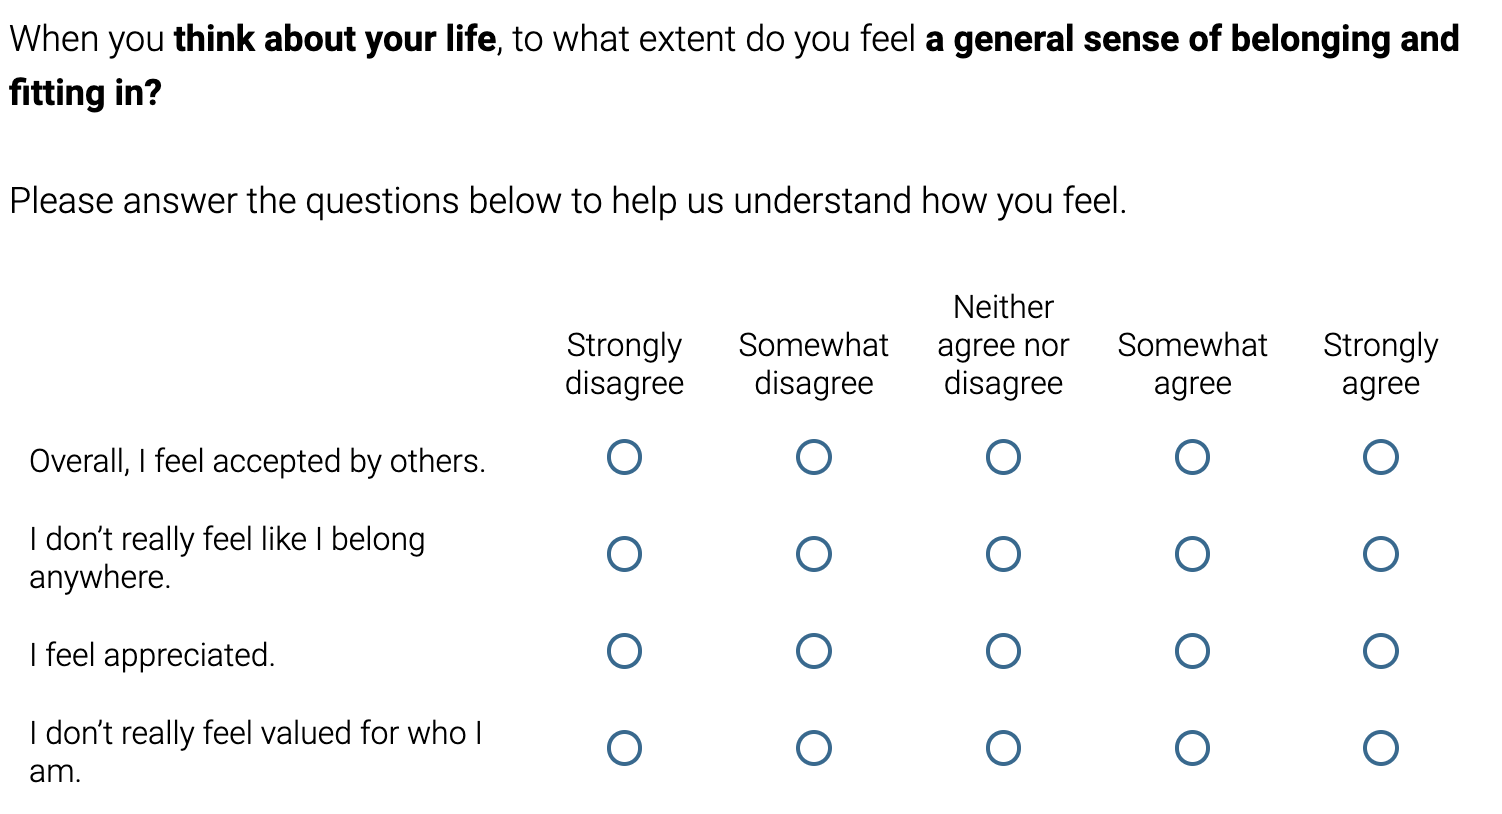
\includegraphics[width=5.01in]{graphics/GlobalTraitPreview} \caption{Preview of the first four items as they appeared in Qualtrics for the global trait form. On the real survey, items were presented in a random order.}\label{fig:qualtrics-preview-global-trait}
\end{figure}

\hypertarget{global-state-form}{%
\section{Global-State Form}\label{global-state-form}}

The items for the global state form of the scale are modified to include the timeframe for the desired measurement. In our validation studies, we asked participants about the past two weeks, as shown in Table \ref{tab:global-state-items}. They were preceded by these instructions:

\begin{quote}
When you \textbf{think about your life at this moment,} to what extent do you feel \textbf{a general sense of belonging and fitting in?}
\end{quote}

\begin{quote}
\textbf{Think back over the past two weeks} and answer the questions below based \textbf{just on your feelings over the past two weeks.}
\end{quote}

This timeframe is, in theory, flexible. For example, one could phrase the scale to ask about the past 30 minutes. This feature might be useful for assessing belonging after an experimental manipulation or a program session.

The response scale was the same as for the global trait items in Section \ref{global-trait}.

\global\setlength{\Oldarrayrulewidth}{\arrayrulewidth}

\global\setlength{\Oldtabcolsep}{\tabcolsep}

\setlength{\tabcolsep}{0pt}

\renewcommand*{\arraystretch}{1.5}



\providecommand{\ascline}[3]{\noalign{\global\arrayrulewidth #1}\arrayrulecolor[HTML]{#2}\cline{#3}}

\begin{longtable}[c]{|p{0.75in}|p{4.00in}}

\caption{SBS-8\ \&\ SBS-16\ items\ in\ the\ global-state\ form.}\label{tab:global-state-items}\\

\ascline{1.5pt}{666666}{1-2}

\multicolumn{1}{>{\raggedleft}m{\dimexpr 0.75in+0\tabcolsep}}{\textcolor[HTML]{000000}{\fontsize{11}{11}\selectfont{\global\setmainfont{Helvetica}{Item\ Number}}}} & \multicolumn{1}{>{\raggedright}m{\dimexpr 4in+0\tabcolsep}}{\textcolor[HTML]{000000}{\fontsize{11}{11}\selectfont{\global\setmainfont{Helvetica}{Item}}}} \\

\ascline{1.5pt}{666666}{1-2}\endfirsthead \caption[]{SBS-8\ \&\ SBS-16\ items\ in\ the\ global-state\ form.}\label{tab:global-state-items}\\

\ascline{1.5pt}{666666}{1-2}

\multicolumn{1}{>{\raggedleft}m{\dimexpr 0.75in+0\tabcolsep}}{\textcolor[HTML]{000000}{\fontsize{11}{11}\selectfont{\global\setmainfont{Helvetica}{Item\ Number}}}} & \multicolumn{1}{>{\raggedright}m{\dimexpr 4in+0\tabcolsep}}{\textcolor[HTML]{000000}{\fontsize{11}{11}\selectfont{\global\setmainfont{Helvetica}{Item}}}} \\

\ascline{1.5pt}{666666}{1-2}\endhead



\multicolumn{2}{>{\raggedright}m{\dimexpr 4.75in+2\tabcolsep}}{\textcolor[HTML]{000000}{\fontsize{11}{11}\selectfont{\global\setmainfont{Helvetica}{Items\ 1-8,\ shown\ in\ the\ top\ half\ of\ the\ table,\ comprise\ the\ 8-item\ version.\ The\ "full"\ scale\ is\ comprised\ of\ all\ 16\ items.}}}} \\

\endfoot



\multicolumn{1}{>{\raggedleft}m{\dimexpr 0.75in+0\tabcolsep}}{\textcolor[HTML]{000000}{\fontsize{11}{11}\selectfont{\global\setmainfont{Helvetica}{1}}}} & \multicolumn{1}{>{\raggedright}m{\dimexpr 4in+0\tabcolsep}}{\textcolor[HTML]{000000}{\fontsize{11}{11}\selectfont{\global\setmainfont{Helvetica}{In\ the\ past\ two\ weeks,\ I\ felt\ a\ sense\ of\ belonging.}}}} \\





\multicolumn{1}{>{\raggedleft}m{\dimexpr 0.75in+0\tabcolsep}}{\textcolor[HTML]{000000}{\fontsize{11}{11}\selectfont{\global\setmainfont{Helvetica}{2}}}} & \multicolumn{1}{>{\raggedright}m{\dimexpr 4in+0\tabcolsep}}{\textcolor[HTML]{000000}{\fontsize{11}{11}\selectfont{\global\setmainfont{Helvetica}{In\ the\ past\ two\ weeks,\ I\ didn't\ really\ feel\ accepted.}}}} \\





\multicolumn{1}{>{\raggedleft}m{\dimexpr 0.75in+0\tabcolsep}}{\textcolor[HTML]{000000}{\fontsize{11}{11}\selectfont{\global\setmainfont{Helvetica}{3}}}} & \multicolumn{1}{>{\raggedright}m{\dimexpr 4in+0\tabcolsep}}{\textcolor[HTML]{000000}{\fontsize{11}{11}\selectfont{\global\setmainfont{Helvetica}{In\ the\ past\ two\ weeks,\ I\ felt\ valued\ by\ others.}}}} \\





\multicolumn{1}{>{\raggedleft}m{\dimexpr 0.75in+0\tabcolsep}}{\textcolor[HTML]{000000}{\fontsize{11}{11}\selectfont{\global\setmainfont{Helvetica}{4}}}} & \multicolumn{1}{>{\raggedright}m{\dimexpr 4in+0\tabcolsep}}{\textcolor[HTML]{000000}{\fontsize{11}{11}\selectfont{\global\setmainfont{Helvetica}{In\ the\ past\ two\ weeks,\ I\ felt\ disregarded.}}}} \\





\multicolumn{1}{>{\raggedleft}m{\dimexpr 0.75in+0\tabcolsep}}{\textcolor[HTML]{000000}{\fontsize{11}{11}\selectfont{\global\setmainfont{Helvetica}{5}}}} & \multicolumn{1}{>{\raggedright}m{\dimexpr 4in+0\tabcolsep}}{\textcolor[HTML]{000000}{\fontsize{11}{11}\selectfont{\global\setmainfont{Helvetica}{In\ the\ past\ two\ weeks,\ I\ felt\ like\ I\ fit\ in.}}}} \\





\multicolumn{1}{>{\raggedleft}m{\dimexpr 0.75in+0\tabcolsep}}{\textcolor[HTML]{000000}{\fontsize{11}{11}\selectfont{\global\setmainfont{Helvetica}{6}}}} & \multicolumn{1}{>{\raggedright}m{\dimexpr 4in+0\tabcolsep}}{\textcolor[HTML]{000000}{\fontsize{11}{11}\selectfont{\global\setmainfont{Helvetica}{In\ the\ past\ two\ weeks,\ I\ felt\ like\ I\ don’t\ really\ fit\ in\ with\ others.}}}} \\





\multicolumn{1}{>{\raggedleft}m{\dimexpr 0.75in+0\tabcolsep}}{\textcolor[HTML]{000000}{\fontsize{11}{11}\selectfont{\global\setmainfont{Helvetica}{7}}}} & \multicolumn{1}{>{\raggedright}m{\dimexpr 4in+0\tabcolsep}}{\textcolor[HTML]{000000}{\fontsize{11}{11}\selectfont{\global\setmainfont{Helvetica}{In\ the\ past\ two\ weeks,\ I\ felt\ connected\ with\ others.}}}} \\





\multicolumn{1}{>{\raggedleft}m{\dimexpr 0.75in+0\tabcolsep}}{\textcolor[HTML]{000000}{\fontsize{11}{11}\selectfont{\global\setmainfont{Helvetica}{8}}}} & \multicolumn{1}{>{\raggedright}m{\dimexpr 4in+0\tabcolsep}}{\textcolor[HTML]{000000}{\fontsize{11}{11}\selectfont{\global\setmainfont{Helvetica}{In\ the\ past\ two\ weeks,\ I\ felt\ so\ distant\ from\ others.}}}} \\

\ascline{1pt}{666666}{1-2}



\multicolumn{1}{>{\raggedleft}m{\dimexpr 0.75in+0\tabcolsep}}{\textcolor[HTML]{000000}{\fontsize{11}{11}\selectfont{\global\setmainfont{Helvetica}{9}}}} & \multicolumn{1}{>{\raggedright}m{\dimexpr 4in+0\tabcolsep}}{\textcolor[HTML]{000000}{\fontsize{11}{11}\selectfont{\global\setmainfont{Helvetica}{In\ the\ past\ two\ weeks,\ I\ felt\ accepted\ by\ others.}}}} \\





\multicolumn{1}{>{\raggedleft}m{\dimexpr 0.75in+0\tabcolsep}}{\textcolor[HTML]{000000}{\fontsize{11}{11}\selectfont{\global\setmainfont{Helvetica}{10}}}} & \multicolumn{1}{>{\raggedright}m{\dimexpr 4in+0\tabcolsep}}{\textcolor[HTML]{000000}{\fontsize{11}{11}\selectfont{\global\setmainfont{Helvetica}{In\ the\ past\ two\ weeks,\ I\ didn’t\ really\ feel\ like\ I\ belonged\ anywhere.}}}} \\





\multicolumn{1}{>{\raggedleft}m{\dimexpr 0.75in+0\tabcolsep}}{\textcolor[HTML]{000000}{\fontsize{11}{11}\selectfont{\global\setmainfont{Helvetica}{11}}}} & \multicolumn{1}{>{\raggedright}m{\dimexpr 4in+0\tabcolsep}}{\textcolor[HTML]{000000}{\fontsize{11}{11}\selectfont{\global\setmainfont{Helvetica}{In\ the\ past\ two\ weeks,\ I\ felt\ appreciated.}}}} \\





\multicolumn{1}{>{\raggedleft}m{\dimexpr 0.75in+0\tabcolsep}}{\textcolor[HTML]{000000}{\fontsize{11}{11}\selectfont{\global\setmainfont{Helvetica}{12}}}} & \multicolumn{1}{>{\raggedright}m{\dimexpr 4in+0\tabcolsep}}{\textcolor[HTML]{000000}{\fontsize{11}{11}\selectfont{\global\setmainfont{Helvetica}{In\ the\ past\ two\ weeks,\ I\ didn’t\ really\ feel\ valued\ for\ who\ I\ am.}}}} \\





\multicolumn{1}{>{\raggedleft}m{\dimexpr 0.75in+0\tabcolsep}}{\textcolor[HTML]{000000}{\fontsize{11}{11}\selectfont{\global\setmainfont{Helvetica}{13}}}} & \multicolumn{1}{>{\raggedright}m{\dimexpr 4in+0\tabcolsep}}{\textcolor[HTML]{000000}{\fontsize{11}{11}\selectfont{\global\setmainfont{Helvetica}{In\ the\ past\ two\ weeks,\ I\ felt\ at\ home\ in\ the\ world.}}}} \\





\multicolumn{1}{>{\raggedleft}m{\dimexpr 0.75in+0\tabcolsep}}{\textcolor[HTML]{000000}{\fontsize{11}{11}\selectfont{\global\setmainfont{Helvetica}{14}}}} & \multicolumn{1}{>{\raggedright}m{\dimexpr 4in+0\tabcolsep}}{\textcolor[HTML]{000000}{\fontsize{11}{11}\selectfont{\global\setmainfont{Helvetica}{In\ the\ past\ two\ weeks,\ I\ felt\ like\ a\ piece\ of\ a\ jig-saw\ puzzle\ that\ doesn’t\ fit\ into\ the\ puzzle.}}}} \\





\multicolumn{1}{>{\raggedleft}m{\dimexpr 0.75in+0\tabcolsep}}{\textcolor[HTML]{000000}{\fontsize{11}{11}\selectfont{\global\setmainfont{Helvetica}{15}}}} & \multicolumn{1}{>{\raggedright}m{\dimexpr 4in+0\tabcolsep}}{\textcolor[HTML]{000000}{\fontsize{11}{11}\selectfont{\global\setmainfont{Helvetica}{In\ the\ past\ two\ weeks,\ I\ felt\ welcome.}}}} \\





\multicolumn{1}{>{\raggedleft}m{\dimexpr 0.75in+0\tabcolsep}}{\textcolor[HTML]{000000}{\fontsize{11}{11}\selectfont{\global\setmainfont{Helvetica}{16}}}} & \multicolumn{1}{>{\raggedright}m{\dimexpr 4in+0\tabcolsep}}{\textcolor[HTML]{000000}{\fontsize{11}{11}\selectfont{\global\setmainfont{Helvetica}{In\ the\ past\ two\ weeks,\ I\ felt\ disconnected\ from\ the\ world\ around\ me.}}}} \\

\ascline{1.5pt}{666666}{1-2}



\end{longtable}



\arrayrulecolor[HTML]{000000}

\global\setlength{\arrayrulewidth}{\Oldarrayrulewidth}

\global\setlength{\tabcolsep}{\Oldtabcolsep}

\renewcommand*{\arraystretch}{1}

\hypertarget{specific-trait-form}{%
\section{Specific Trait Form}\label{specific-trait-form}}

The items for any specific form of the scale will be tailored for the identity or context in question. We validated the scale for a university student identity. The instructions were:

\begin{quote}
Think about \textbf{your entire college career.} When you think about \textbf{your time as a student at the University of XXX,} to what extent do you feel \textbf{a sense of belonging and fitting in? }
\end{quote}

\begin{quote}
Please answer the questions below to help us understand how you feel.
\end{quote}

Note the reference to their \emph{specific} identity and the unbounded \emph{trait} timeframe.

The response scale was the same as for the global trait items in Section \ref{global-trait}.

\global\setlength{\Oldarrayrulewidth}{\arrayrulewidth}

\global\setlength{\Oldtabcolsep}{\tabcolsep}

\setlength{\tabcolsep}{0pt}

\renewcommand*{\arraystretch}{1.5}



\providecommand{\ascline}[3]{\noalign{\global\arrayrulewidth #1}\arrayrulecolor[HTML]{#2}\cline{#3}}

\begin{longtable}[c]{|p{0.75in}|p{4.00in}}

\caption{SBS-8\ \&\ SBS-16\ items\ in\ the\ specific-trait\ form.}\label{tab:specific-trait-items}\\

\ascline{1.5pt}{666666}{1-2}

\multicolumn{1}{>{\raggedleft}m{\dimexpr 0.75in+0\tabcolsep}}{\textcolor[HTML]{000000}{\fontsize{11}{11}\selectfont{\global\setmainfont{Helvetica}{Item\ Number}}}} & \multicolumn{1}{>{\raggedright}m{\dimexpr 4in+0\tabcolsep}}{\textcolor[HTML]{000000}{\fontsize{11}{11}\selectfont{\global\setmainfont{Helvetica}{Item}}}} \\

\ascline{1.5pt}{666666}{1-2}\endfirsthead \caption[]{SBS-8\ \&\ SBS-16\ items\ in\ the\ specific-trait\ form.}\label{tab:specific-trait-items}\\

\ascline{1.5pt}{666666}{1-2}

\multicolumn{1}{>{\raggedleft}m{\dimexpr 0.75in+0\tabcolsep}}{\textcolor[HTML]{000000}{\fontsize{11}{11}\selectfont{\global\setmainfont{Helvetica}{Item\ Number}}}} & \multicolumn{1}{>{\raggedright}m{\dimexpr 4in+0\tabcolsep}}{\textcolor[HTML]{000000}{\fontsize{11}{11}\selectfont{\global\setmainfont{Helvetica}{Item}}}} \\

\ascline{1.5pt}{666666}{1-2}\endhead



\multicolumn{2}{>{\raggedright}m{\dimexpr 4.75in+2\tabcolsep}}{\textcolor[HTML]{000000}{\fontsize{11}{11}\selectfont{\global\setmainfont{Helvetica}{Items\ 1-8,\ shown\ in\ the\ top\ half\ of\ the\ table,\ comprise\ the\ 8-item\ version.\ The\ "full"\ scale\ is\ comprised\ of\ all\ 16\ items.}}}} \\

\endfoot



\multicolumn{1}{>{\raggedleft}m{\dimexpr 0.75in+0\tabcolsep}}{\textcolor[HTML]{000000}{\fontsize{11}{11}\selectfont{\global\setmainfont{Helvetica}{1}}}} & \multicolumn{1}{>{\raggedright}m{\dimexpr 4in+0\tabcolsep}}{\textcolor[HTML]{000000}{\fontsize{11}{11}\selectfont{\global\setmainfont{Helvetica}{In\ general,\ as\ a\ student\ at\ XXX,\ I\ feel\ a\ sense\ of\ belonging.}}}} \\





\multicolumn{1}{>{\raggedleft}m{\dimexpr 0.75in+0\tabcolsep}}{\textcolor[HTML]{000000}{\fontsize{11}{11}\selectfont{\global\setmainfont{Helvetica}{2}}}} & \multicolumn{1}{>{\raggedright}m{\dimexpr 4in+0\tabcolsep}}{\textcolor[HTML]{000000}{\fontsize{11}{11}\selectfont{\global\setmainfont{Helvetica}{As\ a\ student\ at\ XXX,\ I\ don't\ really\ feel\ accepted.}}}} \\





\multicolumn{1}{>{\raggedleft}m{\dimexpr 0.75in+0\tabcolsep}}{\textcolor[HTML]{000000}{\fontsize{11}{11}\selectfont{\global\setmainfont{Helvetica}{3}}}} & \multicolumn{1}{>{\raggedright}m{\dimexpr 4in+0\tabcolsep}}{\textcolor[HTML]{000000}{\fontsize{11}{11}\selectfont{\global\setmainfont{Helvetica}{Overall,\ I\ feel\ valued\ by\ other\ students\ at\ XXX}}}} \\





\multicolumn{1}{>{\raggedleft}m{\dimexpr 0.75in+0\tabcolsep}}{\textcolor[HTML]{000000}{\fontsize{11}{11}\selectfont{\global\setmainfont{Helvetica}{4}}}} & \multicolumn{1}{>{\raggedright}m{\dimexpr 4in+0\tabcolsep}}{\textcolor[HTML]{000000}{\fontsize{11}{11}\selectfont{\global\setmainfont{Helvetica}{As\ a\ student\ at\ XXX,\ I\ feel\ disregarded.}}}} \\





\multicolumn{1}{>{\raggedleft}m{\dimexpr 0.75in+0\tabcolsep}}{\textcolor[HTML]{000000}{\fontsize{11}{11}\selectfont{\global\setmainfont{Helvetica}{5}}}} & \multicolumn{1}{>{\raggedright}m{\dimexpr 4in+0\tabcolsep}}{\textcolor[HTML]{000000}{\fontsize{11}{11}\selectfont{\global\setmainfont{Helvetica}{As\ a\ student\ at\ XXX,\ I\ feel\ like\ I\ fit\ in.}}}} \\





\multicolumn{1}{>{\raggedleft}m{\dimexpr 0.75in+0\tabcolsep}}{\textcolor[HTML]{000000}{\fontsize{11}{11}\selectfont{\global\setmainfont{Helvetica}{6}}}} & \multicolumn{1}{>{\raggedright}m{\dimexpr 4in+0\tabcolsep}}{\textcolor[HTML]{000000}{\fontsize{11}{11}\selectfont{\global\setmainfont{Helvetica}{I\ feel\ like\ I\ don’t\ really\ fit\ in\ with\ other\ students\ at\ XXX}}}} \\





\multicolumn{1}{>{\raggedleft}m{\dimexpr 0.75in+0\tabcolsep}}{\textcolor[HTML]{000000}{\fontsize{11}{11}\selectfont{\global\setmainfont{Helvetica}{7}}}} & \multicolumn{1}{>{\raggedright}m{\dimexpr 4in+0\tabcolsep}}{\textcolor[HTML]{000000}{\fontsize{11}{11}\selectfont{\global\setmainfont{Helvetica}{I\ feel\ connected\ with\ other\ students\ at\ XXX.}}}} \\





\multicolumn{1}{>{\raggedleft}m{\dimexpr 0.75in+0\tabcolsep}}{\textcolor[HTML]{000000}{\fontsize{11}{11}\selectfont{\global\setmainfont{Helvetica}{8}}}} & \multicolumn{1}{>{\raggedright}m{\dimexpr 4in+0\tabcolsep}}{\textcolor[HTML]{000000}{\fontsize{11}{11}\selectfont{\global\setmainfont{Helvetica}{I\ feel\ so\ distant\ from\ other\ students\ at\ XXX.}}}} \\

\ascline{1pt}{666666}{1-2}



\multicolumn{1}{>{\raggedleft}m{\dimexpr 0.75in+0\tabcolsep}}{\textcolor[HTML]{000000}{\fontsize{11}{11}\selectfont{\global\setmainfont{Helvetica}{9}}}} & \multicolumn{1}{>{\raggedright}m{\dimexpr 4in+0\tabcolsep}}{\textcolor[HTML]{000000}{\fontsize{11}{11}\selectfont{\global\setmainfont{Helvetica}{Overall,\ as\ a\ student\ at\ XXX\ I\ feel\ accepted\ by\ others.}}}} \\





\multicolumn{1}{>{\raggedleft}m{\dimexpr 0.75in+0\tabcolsep}}{\textcolor[HTML]{000000}{\fontsize{11}{11}\selectfont{\global\setmainfont{Helvetica}{10}}}} & \multicolumn{1}{>{\raggedright}m{\dimexpr 4in+0\tabcolsep}}{\textcolor[HTML]{000000}{\fontsize{11}{11}\selectfont{\global\setmainfont{Helvetica}{As\ a\ student\ at\ XXX,\ I\ don’t\ really\ feel\ like\ I\ belong\ anywhere.}}}} \\





\multicolumn{1}{>{\raggedleft}m{\dimexpr 0.75in+0\tabcolsep}}{\textcolor[HTML]{000000}{\fontsize{11}{11}\selectfont{\global\setmainfont{Helvetica}{11}}}} & \multicolumn{1}{>{\raggedright}m{\dimexpr 4in+0\tabcolsep}}{\textcolor[HTML]{000000}{\fontsize{11}{11}\selectfont{\global\setmainfont{Helvetica}{As\ a\ student\ at\ XXX,\ I\ feel\ appreciated.}}}} \\





\multicolumn{1}{>{\raggedleft}m{\dimexpr 0.75in+0\tabcolsep}}{\textcolor[HTML]{000000}{\fontsize{11}{11}\selectfont{\global\setmainfont{Helvetica}{12}}}} & \multicolumn{1}{>{\raggedright}m{\dimexpr 4in+0\tabcolsep}}{\textcolor[HTML]{000000}{\fontsize{11}{11}\selectfont{\global\setmainfont{Helvetica}{As\ a\ student\ at\ XXX,\ I\ don’t\ really\ feel\ valued\ for\ who\ I\ am.}}}} \\





\multicolumn{1}{>{\raggedleft}m{\dimexpr 0.75in+0\tabcolsep}}{\textcolor[HTML]{000000}{\fontsize{11}{11}\selectfont{\global\setmainfont{Helvetica}{13}}}} & \multicolumn{1}{>{\raggedright}m{\dimexpr 4in+0\tabcolsep}}{\textcolor[HTML]{000000}{\fontsize{11}{11}\selectfont{\global\setmainfont{Helvetica}{I\ feel\ at\ home\ as\ a\ student\ at\ XXX.}}}} \\





\multicolumn{1}{>{\raggedleft}m{\dimexpr 0.75in+0\tabcolsep}}{\textcolor[HTML]{000000}{\fontsize{11}{11}\selectfont{\global\setmainfont{Helvetica}{14}}}} & \multicolumn{1}{>{\raggedright}m{\dimexpr 4in+0\tabcolsep}}{\textcolor[HTML]{000000}{\fontsize{11}{11}\selectfont{\global\setmainfont{Helvetica}{As\ a\ student\ at\ XXX,\ I\ feel\ like\ a\ piece\ of\ a\ jig-saw\ puzzle\ that\ doesn’t\ fit\ into\ the\ puzzle.}}}} \\





\multicolumn{1}{>{\raggedleft}m{\dimexpr 0.75in+0\tabcolsep}}{\textcolor[HTML]{000000}{\fontsize{11}{11}\selectfont{\global\setmainfont{Helvetica}{15}}}} & \multicolumn{1}{>{\raggedright}m{\dimexpr 4in+0\tabcolsep}}{\textcolor[HTML]{000000}{\fontsize{11}{11}\selectfont{\global\setmainfont{Helvetica}{In\ general,\ as\ a\ student\ at\ XXX,\ I\ feel\ welcome.}}}} \\





\multicolumn{1}{>{\raggedleft}m{\dimexpr 0.75in+0\tabcolsep}}{\textcolor[HTML]{000000}{\fontsize{11}{11}\selectfont{\global\setmainfont{Helvetica}{16}}}} & \multicolumn{1}{>{\raggedright}m{\dimexpr 4in+0\tabcolsep}}{\textcolor[HTML]{000000}{\fontsize{11}{11}\selectfont{\global\setmainfont{Helvetica}{I\ feel\ disconnected\ from\ students\ at\ XXX.}}}} \\

\ascline{1.5pt}{666666}{1-2}



\end{longtable}



\arrayrulecolor[HTML]{000000}

\global\setlength{\arrayrulewidth}{\Oldarrayrulewidth}

\global\setlength{\tabcolsep}{\Oldtabcolsep}

\renewcommand*{\arraystretch}{1}

\hypertarget{specific-state-form}{%
\section{Specific State Form}\label{specific-state-form}}

This form of the scale requires a \emph{specific} identity and a constrained timeframe for the \emph{state} measurement. Both elements can be adapted as necessary.

\begin{quote}
When you think about being a \textbf{student at the University of XXX at this moment,} to what extent do you feel a sense of belonging and fitting in?
\end{quote}

\begin{quote}
\textbf{Think back over the past two weeks} and answer the questions below based on your feelings about being a \textbf{student at XXX over just the past two weeks.}
\end{quote}

Note the reference to their \emph{specific} identity and the bounded \emph{state} timeframe.

The response scale was the same as for the global trait items in Section \ref{global-trait}.

\global\setlength{\Oldarrayrulewidth}{\arrayrulewidth}

\global\setlength{\Oldtabcolsep}{\tabcolsep}

\setlength{\tabcolsep}{0pt}

\renewcommand*{\arraystretch}{1.5}



\providecommand{\ascline}[3]{\noalign{\global\arrayrulewidth #1}\arrayrulecolor[HTML]{#2}\cline{#3}}

\begin{longtable}[c]{|p{0.75in}|p{4.00in}}

\caption{SBS-8\ \&\ SBS-16\ items\ in\ the\ specific-trait\ form.}\label{tab:specific-trait-items}\\

\ascline{1.5pt}{666666}{1-2}

\multicolumn{1}{>{\raggedleft}m{\dimexpr 0.75in+0\tabcolsep}}{\textcolor[HTML]{000000}{\fontsize{11}{11}\selectfont{\global\setmainfont{Helvetica}{Item\ Number}}}} & \multicolumn{1}{>{\raggedright}m{\dimexpr 4in+0\tabcolsep}}{\textcolor[HTML]{000000}{\fontsize{11}{11}\selectfont{\global\setmainfont{Helvetica}{Item}}}} \\

\ascline{1.5pt}{666666}{1-2}\endfirsthead \caption[]{SBS-8\ \&\ SBS-16\ items\ in\ the\ specific-trait\ form.}\label{tab:specific-trait-items}\\

\ascline{1.5pt}{666666}{1-2}

\multicolumn{1}{>{\raggedleft}m{\dimexpr 0.75in+0\tabcolsep}}{\textcolor[HTML]{000000}{\fontsize{11}{11}\selectfont{\global\setmainfont{Helvetica}{Item\ Number}}}} & \multicolumn{1}{>{\raggedright}m{\dimexpr 4in+0\tabcolsep}}{\textcolor[HTML]{000000}{\fontsize{11}{11}\selectfont{\global\setmainfont{Helvetica}{Item}}}} \\

\ascline{1.5pt}{666666}{1-2}\endhead



\multicolumn{2}{>{\raggedright}m{\dimexpr 4.75in+2\tabcolsep}}{\textcolor[HTML]{000000}{\fontsize{11}{11}\selectfont{\global\setmainfont{Helvetica}{Items\ 1-8,\ shown\ in\ the\ top\ half\ of\ the\ table,\ comprise\ the\ 8-item\ version.\ The\ "full"\ scale\ is\ comprised\ of\ all\ 16\ items.}}}} \\

\endfoot



\multicolumn{1}{>{\raggedleft}m{\dimexpr 0.75in+0\tabcolsep}}{\textcolor[HTML]{000000}{\fontsize{11}{11}\selectfont{\global\setmainfont{Helvetica}{1}}}} & \multicolumn{1}{>{\raggedright}m{\dimexpr 4in+0\tabcolsep}}{\textcolor[HTML]{000000}{\fontsize{11}{11}\selectfont{\global\setmainfont{Helvetica}{In\ the\ past\ two\ weeks,\ as\ a\ student\ at\ XXX,\ I\ felt\ a\ sense\ of\ belonging.}}}} \\





\multicolumn{1}{>{\raggedleft}m{\dimexpr 0.75in+0\tabcolsep}}{\textcolor[HTML]{000000}{\fontsize{11}{11}\selectfont{\global\setmainfont{Helvetica}{2}}}} & \multicolumn{1}{>{\raggedright}m{\dimexpr 4in+0\tabcolsep}}{\textcolor[HTML]{000000}{\fontsize{11}{11}\selectfont{\global\setmainfont{Helvetica}{In\ the\ past\ two\ weeks,\ as\ a\ student\ at\ XXX,\ I\ didn't\ really\ feel\ accepted.}}}} \\





\multicolumn{1}{>{\raggedleft}m{\dimexpr 0.75in+0\tabcolsep}}{\textcolor[HTML]{000000}{\fontsize{11}{11}\selectfont{\global\setmainfont{Helvetica}{3}}}} & \multicolumn{1}{>{\raggedright}m{\dimexpr 4in+0\tabcolsep}}{\textcolor[HTML]{000000}{\fontsize{11}{11}\selectfont{\global\setmainfont{Helvetica}{In\ the\ past\ two\ weeks,\ I\ felt\ valued\ by\ other\ students\ at\ XXX}}}} \\





\multicolumn{1}{>{\raggedleft}m{\dimexpr 0.75in+0\tabcolsep}}{\textcolor[HTML]{000000}{\fontsize{11}{11}\selectfont{\global\setmainfont{Helvetica}{4}}}} & \multicolumn{1}{>{\raggedright}m{\dimexpr 4in+0\tabcolsep}}{\textcolor[HTML]{000000}{\fontsize{11}{11}\selectfont{\global\setmainfont{Helvetica}{In\ the\ past\ two\ weeks,\ as\ a\ student\ at\ XXX,\ I\ felt\ disregarded.}}}} \\





\multicolumn{1}{>{\raggedleft}m{\dimexpr 0.75in+0\tabcolsep}}{\textcolor[HTML]{000000}{\fontsize{11}{11}\selectfont{\global\setmainfont{Helvetica}{5}}}} & \multicolumn{1}{>{\raggedright}m{\dimexpr 4in+0\tabcolsep}}{\textcolor[HTML]{000000}{\fontsize{11}{11}\selectfont{\global\setmainfont{Helvetica}{In\ the\ past\ two\ weeks,\ as\ a\ student\ at\ XXX,\ I\ felt\ like\ I\ fit\ in.}}}} \\





\multicolumn{1}{>{\raggedleft}m{\dimexpr 0.75in+0\tabcolsep}}{\textcolor[HTML]{000000}{\fontsize{11}{11}\selectfont{\global\setmainfont{Helvetica}{6}}}} & \multicolumn{1}{>{\raggedright}m{\dimexpr 4in+0\tabcolsep}}{\textcolor[HTML]{000000}{\fontsize{11}{11}\selectfont{\global\setmainfont{Helvetica}{In\ the\ past\ two\ weeks,\ I\ felt\ like\ I\ didn’t\ really\ fit\ in\ with\ other\ students\ at\ XXX}}}} \\





\multicolumn{1}{>{\raggedleft}m{\dimexpr 0.75in+0\tabcolsep}}{\textcolor[HTML]{000000}{\fontsize{11}{11}\selectfont{\global\setmainfont{Helvetica}{7}}}} & \multicolumn{1}{>{\raggedright}m{\dimexpr 4in+0\tabcolsep}}{\textcolor[HTML]{000000}{\fontsize{11}{11}\selectfont{\global\setmainfont{Helvetica}{In\ the\ past\ two\ weeks,\ I\ felt\ connected\ with\ other\ students\ at\ XXX.}}}} \\





\multicolumn{1}{>{\raggedleft}m{\dimexpr 0.75in+0\tabcolsep}}{\textcolor[HTML]{000000}{\fontsize{11}{11}\selectfont{\global\setmainfont{Helvetica}{8}}}} & \multicolumn{1}{>{\raggedright}m{\dimexpr 4in+0\tabcolsep}}{\textcolor[HTML]{000000}{\fontsize{11}{11}\selectfont{\global\setmainfont{Helvetica}{In\ the\ past\ two\ weeks,\ I\ felt\ so\ distant\ from\ other\ students\ at\ XXX.}}}} \\

\ascline{1pt}{666666}{1-2}



\multicolumn{1}{>{\raggedleft}m{\dimexpr 0.75in+0\tabcolsep}}{\textcolor[HTML]{000000}{\fontsize{11}{11}\selectfont{\global\setmainfont{Helvetica}{9}}}} & \multicolumn{1}{>{\raggedright}m{\dimexpr 4in+0\tabcolsep}}{\textcolor[HTML]{000000}{\fontsize{11}{11}\selectfont{\global\setmainfont{Helvetica}{In\ the\ past\ two\ weeks,\ as\ a\ student\ at\ XXX\ I\ felt\ accepted\ by\ others.}}}} \\





\multicolumn{1}{>{\raggedleft}m{\dimexpr 0.75in+0\tabcolsep}}{\textcolor[HTML]{000000}{\fontsize{11}{11}\selectfont{\global\setmainfont{Helvetica}{10}}}} & \multicolumn{1}{>{\raggedright}m{\dimexpr 4in+0\tabcolsep}}{\textcolor[HTML]{000000}{\fontsize{11}{11}\selectfont{\global\setmainfont{Helvetica}{In\ the\ past\ two\ weeks,\ as\ a\ student\ at\ XXX,\ I\ didn’t\ really\ feel\ like\ I\ belonged\ anywhere.}}}} \\





\multicolumn{1}{>{\raggedleft}m{\dimexpr 0.75in+0\tabcolsep}}{\textcolor[HTML]{000000}{\fontsize{11}{11}\selectfont{\global\setmainfont{Helvetica}{11}}}} & \multicolumn{1}{>{\raggedright}m{\dimexpr 4in+0\tabcolsep}}{\textcolor[HTML]{000000}{\fontsize{11}{11}\selectfont{\global\setmainfont{Helvetica}{In\ the\ past\ two\ weeks,\ as\ a\ student\ at\ XXX,\ I\ felt\ appreciated.}}}} \\





\multicolumn{1}{>{\raggedleft}m{\dimexpr 0.75in+0\tabcolsep}}{\textcolor[HTML]{000000}{\fontsize{11}{11}\selectfont{\global\setmainfont{Helvetica}{12}}}} & \multicolumn{1}{>{\raggedright}m{\dimexpr 4in+0\tabcolsep}}{\textcolor[HTML]{000000}{\fontsize{11}{11}\selectfont{\global\setmainfont{Helvetica}{In\ the\ past\ two\ weeks,\ as\ a\ student\ at\ XXX,\ I\ didn’t\ really\ feel\ valued\ for\ who\ I\ am.}}}} \\





\multicolumn{1}{>{\raggedleft}m{\dimexpr 0.75in+0\tabcolsep}}{\textcolor[HTML]{000000}{\fontsize{11}{11}\selectfont{\global\setmainfont{Helvetica}{13}}}} & \multicolumn{1}{>{\raggedright}m{\dimexpr 4in+0\tabcolsep}}{\textcolor[HTML]{000000}{\fontsize{11}{11}\selectfont{\global\setmainfont{Helvetica}{In\ the\ past\ two\ weeks,\ I\ felt\ at\ home\ as\ a\ student\ at\ XXX.}}}} \\





\multicolumn{1}{>{\raggedleft}m{\dimexpr 0.75in+0\tabcolsep}}{\textcolor[HTML]{000000}{\fontsize{11}{11}\selectfont{\global\setmainfont{Helvetica}{14}}}} & \multicolumn{1}{>{\raggedright}m{\dimexpr 4in+0\tabcolsep}}{\textcolor[HTML]{000000}{\fontsize{11}{11}\selectfont{\global\setmainfont{Helvetica}{In\ the\ past\ two\ weeks,\ as\ a\ student\ at\ XXX,\ I\ felt\ like\ a\ piece\ of\ a\ jig-saw\ puzzle\ that\ doesn’t\ fit\ into\ the\ puzzle.}}}} \\





\multicolumn{1}{>{\raggedleft}m{\dimexpr 0.75in+0\tabcolsep}}{\textcolor[HTML]{000000}{\fontsize{11}{11}\selectfont{\global\setmainfont{Helvetica}{15}}}} & \multicolumn{1}{>{\raggedright}m{\dimexpr 4in+0\tabcolsep}}{\textcolor[HTML]{000000}{\fontsize{11}{11}\selectfont{\global\setmainfont{Helvetica}{In\ the\ past\ two\ weeks,\ as\ a\ student\ at\ XXX,\ I\ felt\ welcome.}}}} \\





\multicolumn{1}{>{\raggedleft}m{\dimexpr 0.75in+0\tabcolsep}}{\textcolor[HTML]{000000}{\fontsize{11}{11}\selectfont{\global\setmainfont{Helvetica}{16}}}} & \multicolumn{1}{>{\raggedright}m{\dimexpr 4in+0\tabcolsep}}{\textcolor[HTML]{000000}{\fontsize{11}{11}\selectfont{\global\setmainfont{Helvetica}{In\ the\ past\ two\ weeks,\ I\ felt\ disconnected\ from\ students\ at\ XXX.}}}} \\

\ascline{1.5pt}{666666}{1-2}



\end{longtable}



\arrayrulecolor[HTML]{000000}

\global\setlength{\arrayrulewidth}{\Oldarrayrulewidth}

\global\setlength{\tabcolsep}{\Oldtabcolsep}

\renewcommand*{\arraystretch}{1}

\end{document}
